\chapter{Project management}
The project was approached using agile methodologies as opposed to the traditional waterfall approach. A main feature of the the approach used in this project was that of test driven development. 

\section{Test Driven Development}

\subsection{Process}

The stages of this process are as follows:
	
\subsubsection*{Write a test}

Firstly a list of tasks needs to be created. This list is made by analysing the requirements of the system and creating a specific task for each feature of the system. 

If there is already a list of tasks then choose one and write a test that can only be passed when the system can carry out the feature as described by the task.


\subsubsection*{Run the test suite}

The entire test suite should be run at this stage with the desired result of all tests passing except for the newly composed test. The new test should fail since the functionality it is testing should not have been implemented at this point. If the test passes then either the functionality was added before the test created, which is not as intended in the TDD process, or it may mean the test is faulty. The test should be reviewed in this case.

If all tests except the new one passes then we can be sure at least that the new test requires some change to the code. This helps reduce the risk of writing tests that pass trivially, which can lead to falsely believing that code is providing functionality that it is not.

\subsubsection*{Code}

In this stage code is written with the aim of passing the test only. No extensions or further functionality should be provided at this point. If the developer becomes aware of the need for expansion then this should be added as a new task. This helps ensure test coverage for all the code.

\subsubsection*{Run test suite again}

The whole test suite is ran again with the aim of all tests passing. If any tests fail then return to the previous step and modify the code. This is repeated until all tests pass.

When all tests are passing then return to stage 1 and choose the next task if any remain.

\begin{figure}[h]
\centering
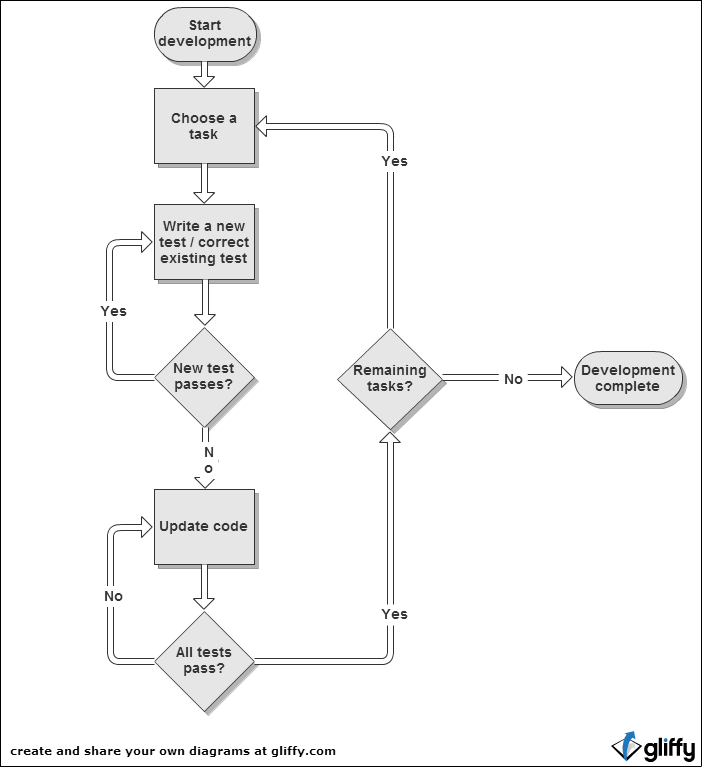
\includegraphics[width=0.9\textwidth]{Images/TDD.png}
\caption{Flowchart of TDD process}
\label{fig:TDD_flowchart}
\end{figure}

\subsection{Advantages of Test Driven Development}

\begin{itemize}
	\item One of the advantages of writing tests before writing code is that you are testing that  the code meets the specification. When tests are created after code is written then there is a chance that the tests will only check that the code functions correctly but not that it meets all the requirements. In the case of TDD great care must be taken with writing the tests so that they accurately reflect the specification and requirements of the system; providing this is the case you can have confidence that the code meets these requirements.

	\item Due to nature of only writing code to pass tests then this inherently leads to good code coverage since all sections of code are covered by at least one test.

	\item Another advantage of TDD is that the passing tests clearly show which tasks have or have not yet been completed. This gives a very good way to accurately monitor progress throughout development.

	\item Finally, as tests are wrote, a test suite is built up which is run whenever code is changed. This means that unexpected affects of a code change are picked up straight away. This can save a lot of time in debugging as when not picked up straight away it can become very time consuming to trace the source of errors. This is especially true if they cause error in other areas which then mask the original source of the error.
\end{itemize}

\subsection{Tools used}

To assist the in the process of TDD I utilised the tools of JUnit and Robotium. JUnit is a testing framework for the Java programming language which assists in the creation and running of automated unit tests. Robotium is a testing framework which facilitates the creation of automated system tests and acceptance tests for the Android platform.

Using a combination of these tools I was able to create a multitude of tests which test individual components and also the interaction between these components. Robotium enabled me to create automated acceptance tests which could carry out tasks from start to finish such as building an entire proof, simulating the use of the graphical user interface by activating button press and touch screen events. Since Robotium simulates using the user interface, I was able to test that not only did the code function correctly but also that users would be able to actually access and use the functions that are offered. Without such automated testing of the graphical features, repeating the tests after each code change would have become a very time consuming process. 





\section{Prioritisation}

Tasks were chosen using the agile principle of structuring and completing tasks in such a way that gives highest value whilst attempting to keep the time frame of delivery small. Use of this principle has a number of advantages. One of these advantages is the modularity of the code developed. Since code is split into tasks with each adding a specific function then code is less dependent on others parts of the system. This reduces complexity, makes testing easier and makes code more reusable. 

Another way this principle was adhered to was by developing code in such a way that at key points the application was operational, but only implementing a subset of the desired functional requirements. An example of this was the design choice of implementing all the necessary requirements so that the system could be fully operational for the language of Propositional Logic before extending it to FOL. The advantages of this are threefold:
\begin{enumerate}
\item In a business situation a product can be delivered to end users at a much earlier date, with non critical functionality being added incrementally.
\item This working application can be used as a prototype. It can be used by people not involved with the development to gain important feedback at an earlier stage than would normally be possible. The feedback may uncover some changes that would improve the user experience, again due to the product being in development it is easier to make changes at this point than it would have been after the project had been fully completed.
\item In the worse case scenario, should unexpected problems arise at a later point which prevents completion of the system then there is still a working application. Despite not meeting all the desired requirements this is certainly better than an application that has attempted to meet all desired requirements but is not actually in a usable state.
\end{enumerate}


\section{Project management tools}

\subsection{Trello}

Following the initial design phase I made use of a web-based project management tool to help facilitate the development process. The tool I used was Trello which follows the Kanban paradigm for software development, a well known agile methodology. Kanban enabled me to visualise the workflow of the project using coloured cards and lists which represented tasks and stages in the workflow respectively. In addition to the tasks, I also created a separate list for bugs. This enabled me to document bugs as soon as they were found without distracting too much from the current task at hand. Bugs were sorted by priority so that the most important issues would be dealt with first.

For each objective I would start by breaking it into smaller tasks. These tasks were then put onto a to-do list on Trello. As each task was then picked for development it would be moved along the  various lists each one representing a stage in the TDD process described earlier.  In addition to the stages described above each task would enter a penultimate stage of further testing; previous tests showed that this task is functioning as required so tests in this stage focused on unusual input intended to cause errors. Finally, when this testing is complete and any discovered errors fixed, the task can be moved into the completed list.

\subsection{Git}

Git is a source code management system. One of the benefits of using Git was that all code and documentation could quickly and easily be uploaded to a remote repository. Since it did not take much time I uploaded the latest version every time a new test was created or passed. This remote repository was used as a backup, so should any data be lost or become inaccessible most of it could easily be recovered from the most recent version.

The version control aspect of this system also meant that previous versions can be restored. In cases  where a bug is accidentally introduced, especially during refactoring, it may be quicker to restore to a previous version rather than spend time debugging the program.

\section{Justification of creating an Android application}

In this section I will discuss the thought process and reasons for choosing to build an application for the Android platform. The reasoning here shall be split into three main choices.

\subsection{Choosing a mobile solution}

One of the first major design choices in this project was to implement the solution for use on a mobile device.  Most people find the best way to learn something new is by doing. My vision for this project was to create a tool that would facilitate interactive learning in a classroom environment. My aim is that the teacher will be able to set an exercise such as asking the students to prove a statement from the given premises. Each student will then be able to tackle the problem at their own pace receiving feedback from the application as they proceed. I decided the best way to achieve these goals was to design a mobile solution.


\begin{figure}[h]
\centering
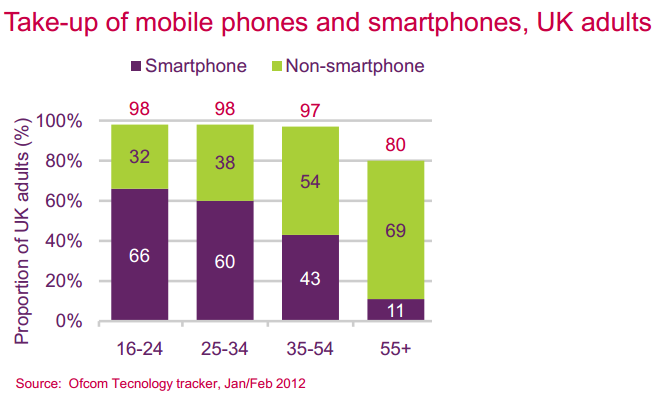
\includegraphics[width=0.9\textwidth]{Images/smartphones.png}
\caption{Smartphone ownership by age}
\label{fig:smartphone_barchart}
\end{figure}

The graph shows that two thirds of people, who are the typical university student age, own smartphones. Furthermore, a fifth of these own a tablet computer. \cite{ofcom} The ownership of mobile technology such as smartphones and tablet computers has been dramatically increasing and it appears that this trend will continue. 
This increasing prevalence of mobile computing devices in our lives contributed to the choice of developing a mobile solution.

\subsection{Choosing a native solution}

The next big choice was to decide whether the implementation should be a mobile web application or a native application. A native application is an application that is wrote to work on a specific platform, whereas a mobile web application can be accessed by multiple platforms using the internet. Of course both solutions have their advantages and disadvantages. The progress being made using HTML5 has meant the distinction between these alternatives have become increasingly vague, even during the time of this project. However, here are some of my resons for the choice I made: 
\begin{itemize}
\item{	
One advantage of the native application is that they are generally faster than their web app counterparts. }
\item{
After the initial download of a native app, access to the internet is no longer necessary. This may be important in a classroom situation where internet connection is not always available.}
\item{
Another advantage of using the native app approach is that they are easy and quick to access. At a click of an icon a user can almost instantly start to use a native app.}
\item{
Finally, native application development is targeted specifically for mobile devices with smaller screens. This makes it easier to create a mobile device interface which utilise features such as touch screen.}
\end{itemize}








\subsection{Choosing the Android platform}

The choice of Android platform was made based mainly on two reasons:

Firstly, as a developer I was already vaguely familiar with Android development and  Java , which is the primary language used in Android development. This familiarity and knowledge allowed me to be asses more accurately, compared to other platforms,  as to what would and would not be possible.

The second and more crucial reason, is the dominance that Android currently holds over the mobile computing market. Figure 2.3 shows the operating systems of mobile devices. 

\begin{figure}[!h]
\centering
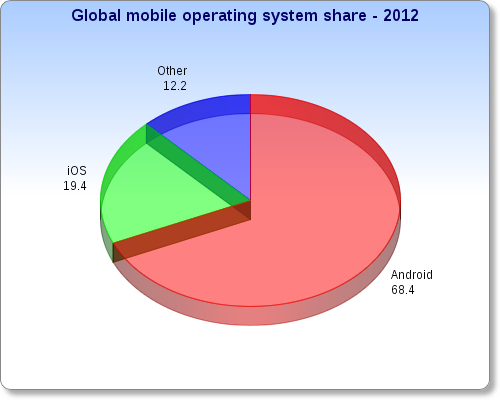
\includegraphics[width=0.9\textwidth]{Images/platform.png}
\caption{Mobile operating system by market share}
\label{fig:operatingsystem_piechart}
\end{figure}

Android has a clear dominance holding almost 70\% of the market share. Since people are most likely to own a device that runs on Android, this was the platform I decided to develop the application for.